\section{Data analysis}
\subsection{Measurement of relaxation times}
Both the spin-spin and the spin-lattice relaxation time have been measured with the use of two different concentrations of Gadolinium solved in water, one solution with 500 water molecules per Gadolinium atom (Gd500) and the other solution containing 600 water molecules per Gadolinium atom (Gd600).
The measured values were acquired by a fit of their respective fit functions (compare equation (\ref{eq:2}) for $T_2$ and equation (\ref{eq:3}) for $T_1$) applied to the measured data as seen in figure \ref{fig:4}

\begin{table}[h]
	\centering
	\begin{tabular}{lll}
		\toprule
		 & Gd500 & Gd600 \\
		\midrule
		$T_2$ & $\left(99.8 \pm 0.5_{stat}\right)\mathrm{ms}$ & $\left(129 \pm 1_{stat}\right)\mathrm{ms}$\\
		
		$T_2$(CP) & $\left(124.0 \pm 0.4_{stat}\right)\mathrm{ms}$ & $\left(150.6 \pm 0.6_{stat}\right)\mathrm{ms}$\\
		
		$T_1$   & $\left(118.8 \pm 2.2_{stat}\right)\mathrm{ms}$ &$ \left(251.9 \pm 4.7_{stat}\right)\mathrm{ms}$\\
		
		\bottomrule
	\end{tabular}
	\caption{Measured Values}
	\label{tab:1}
\end{table}
\noindent
Pulse I has to be maximized in order to represent a 90\textdegree\, pulse, it was set to $\approx 2.1$, and Pulse II has to be minimized in order to be a 180\textdegree, it was set to $\approx 2.2$.
We acquired a data point at $900 \mathrm{ms}$ echo time for the $T_1$ Gd500 measurement which we decided to exclude from the fitted dataset as it was way higher than one would theoretically expect. We found the reason for this to be the sensitivity of the measurement configuration to the background noise, because we changed the integrated over peak window before the acquirement of said data point.
One theoretically expects $T_2$(CP) to be larger than $T_1$ for both solutions,
because the spin-spin interaction dominates $T_2$: Dipoles want to align in the energetically most favorable way, antiparallel. This alignment proceeds faster in comparison to the spin-lattice interaction important for the $T_1$ measurement. $T_1$ describes the average time needed for the mean magnetization to go over from antiparallel to parallel alignment with respect to the external magnetic field, this is microscopically described by single spins orienting themselves from $-1/2$ to $+1/2$.\cite{manual} We observe our expectation of $T_2$ (CP) being larger and more precise than $T_2$, as explained in the theory section \ref{sec:5}, to be true.
\begin{figure}[h]
	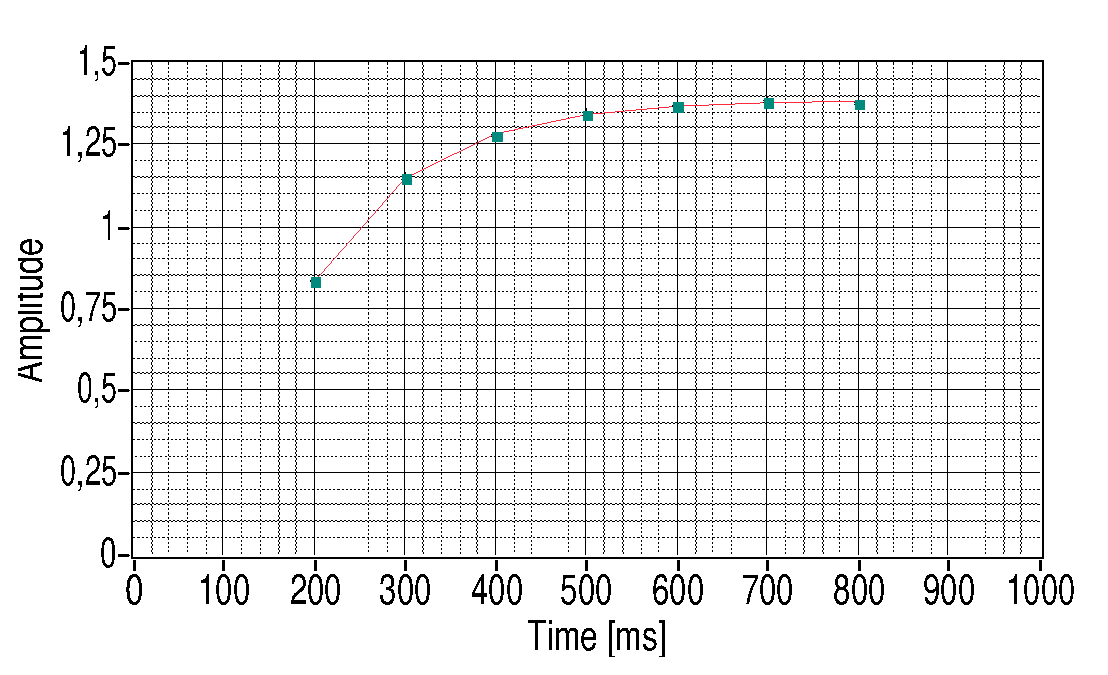
\includegraphics[width=75mm]{GA500T1Fit}
	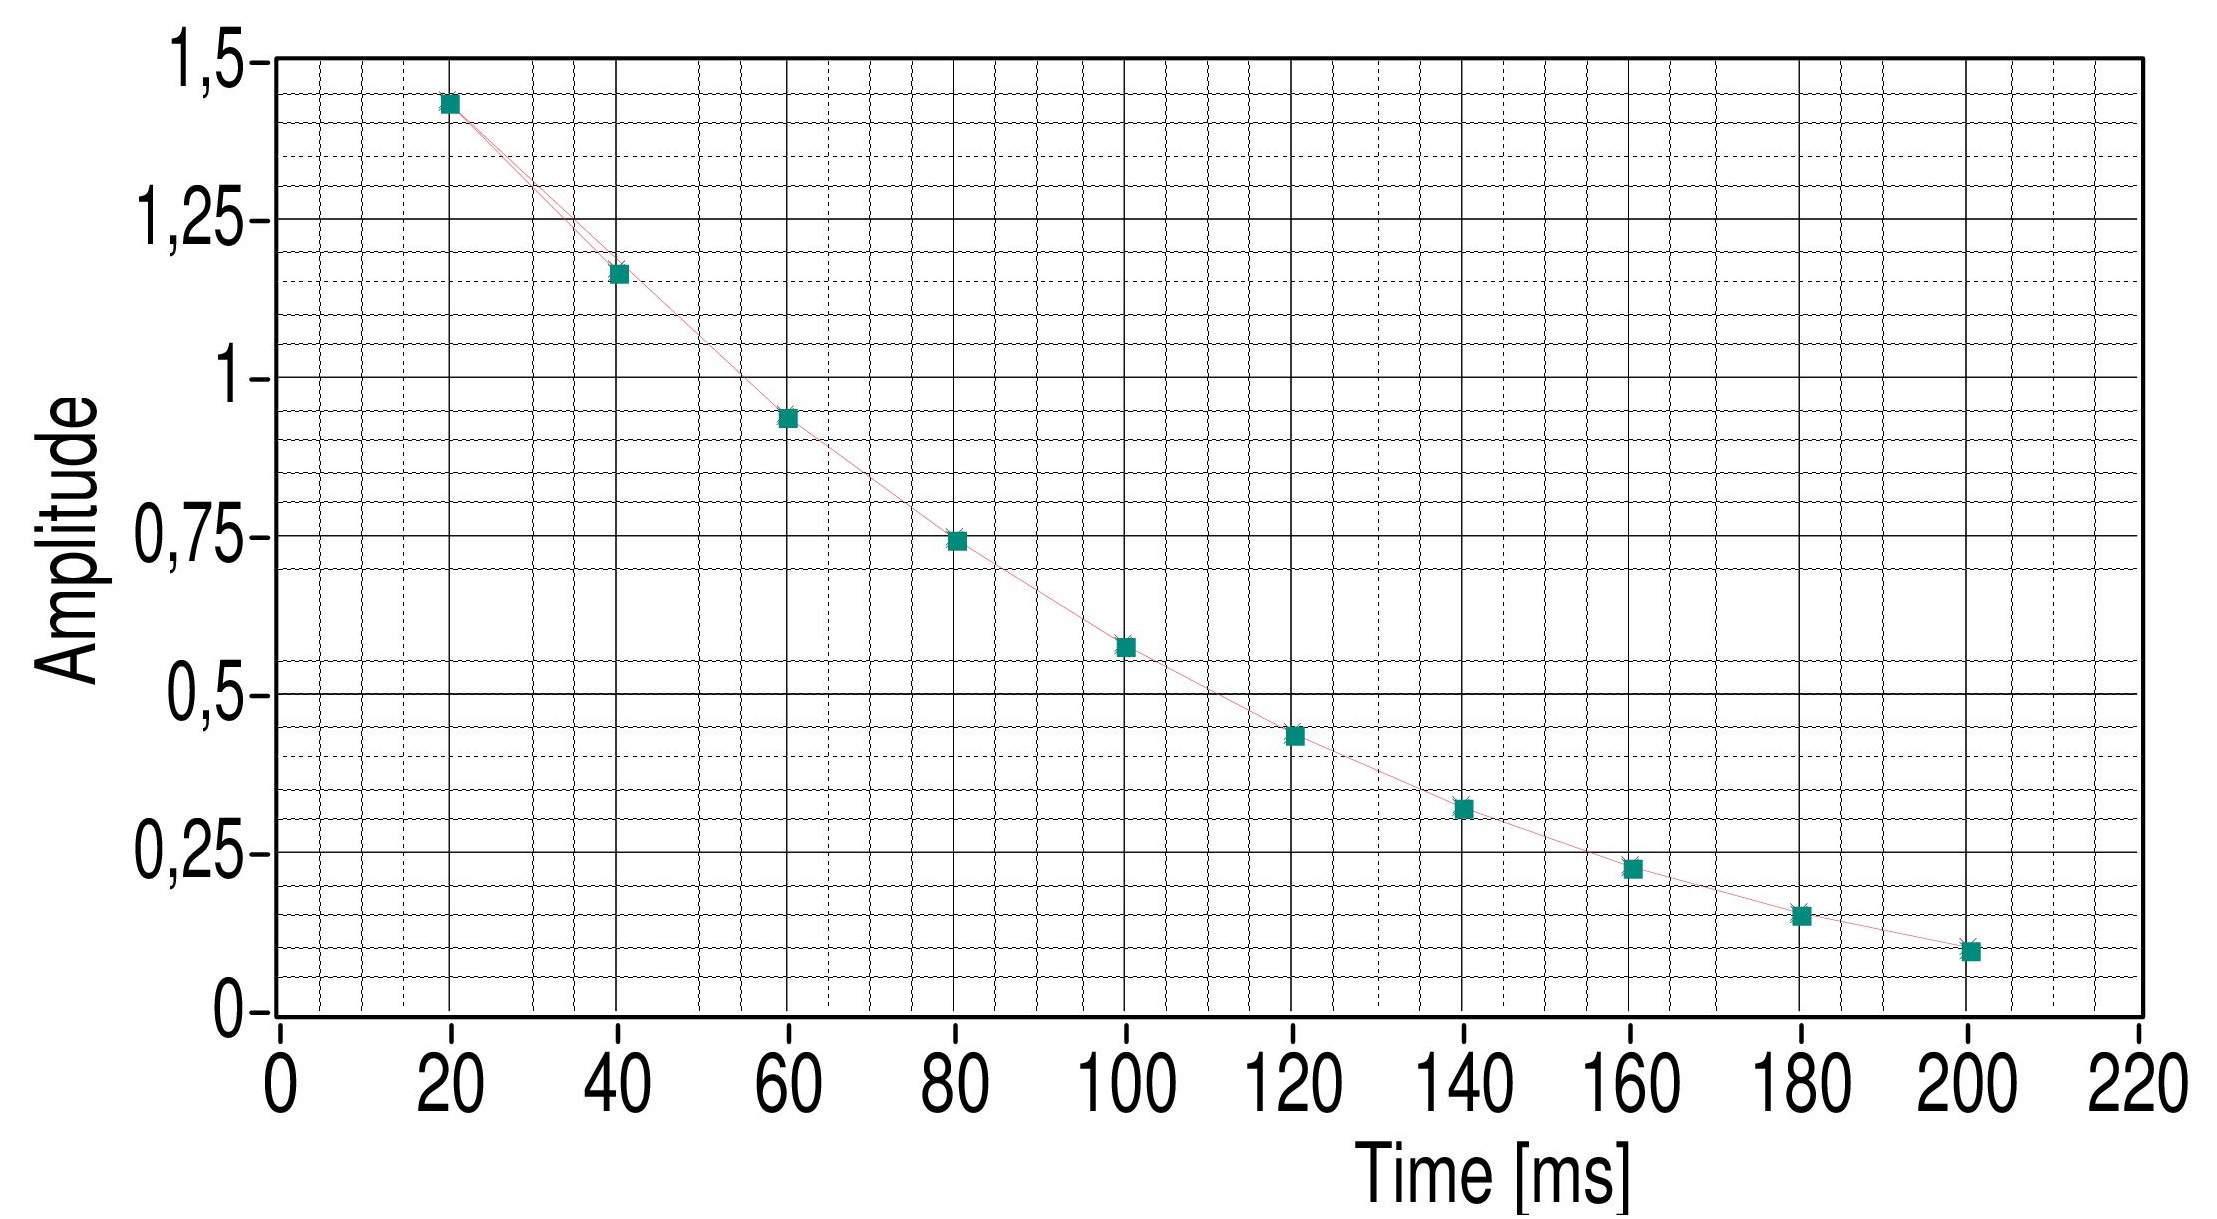
\includegraphics[width=75mm]{Gd500T2Fit}
	\includegraphics*[width=75mm]{Gd500T2CPFit}
	\centering
	\caption{\itshape In the top row: spin-lattice relaxation time $T_1$ in Gd500 with spin-echo method\\
		From left to right in the bottom row: spin-spin relaxation time $T_2$ in Gd500 with spin-echo method and spin-spin relaxation time $T_2$ in Gd500 with the Carr-Purcell (CP) method}
	\label{fig:4}
\end{figure}
\noindent
We furthermore observe the relaxation times of Gd500 to be shorter than for Gd600. Gadolinium is strongly paramagnetic and is magnetized at room temperature (Curie point at $\approx 19$ \textcelsius). The form of paramagnetism exhibited by Gadolinium compounds derives from electrons, not protons, and is known as Curie Paramagnetism. Because of electrons having $s=1/2$, but a much smaller size than the proton, their gyromagnetic ratio is $\approx 657$ times larger. If the electrons remain unpaired in shells or bonding orbitals, the unbalanced spin produce a strong magnetic moment capable of inducing magnetic relaxation in nearby nuclei. The seven unpaired electrons in the $4f \rightarrow s_e = 7/2$ subshell therefore account for the elements strong paramagnetism. \cite{Gadolinium} The presence of such large fluctuating paramagnetic moments in a solution has strong effects on the nuclear spin relaxation of the solvent water nuclei. Therefore, the more Gadolinium atoms available the more dipole-dipole interactions between the water molecules and the Gadolinium atoms are possible and the shorter is the relaxation time.
Instead we measured exactly the opposite to be true as can be seen in table \ref{tab:1}. We therefore repeated our measurement for $T_2$(CP) and for $T_1$ with the Gd600 probe and a more narrow peak window to further exclude background noise. $T_2$(Cp) did not change much, but the new value for $T_1$ increased such that it met our theoretical expectations. We hence replaced the first measured value of $T_1 = \left(135.8 \pm 1.2_{stat}\right)\mathrm{ms}$ with the second measured value in table \ref{tab:1}. Thus, again the use of the same configuration with a slightly more narrow peak window leads to a huge difference in measured values. Furthermore, we excluded the data produced for a spin echo time below $t=200ms$, because the fit could not account for these as they were reflected across the time axis such that the measured values actually started with a decreasing trend until the zero crossing of the amplitude was met at around $t=200ms$. Altogether, the systematic deviation of $T_1$ from our theoretical expectation is due to an incomplete data set and due to the whole setup being very sensitive to the integrated over peak window, which hence should be checked quite thoroughly in order to guarantee reproducibility of results in this section.\\



\subsection{Chemical shift}
In order to identify the different samples A-E with the given chemical substances (Toluene, P-Xylene, Acetic acid, Fluoroacetone, Fluoroacetonitril) we applied a $90$\textdegree\, pulse on the respective samples and acquired via Fourier transformation a frequency spectrum as output signal in which the different Larmor frequencies where observable.
\begin{figure}[h]
	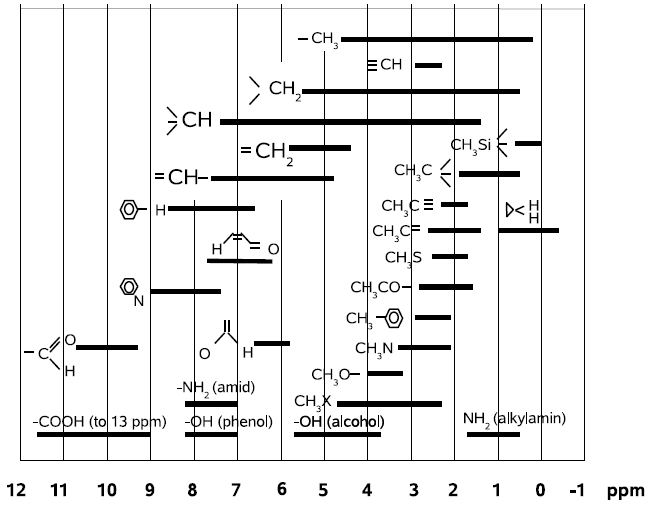
\includegraphics[width=100mm]{Calibration}
	\centering
	\caption{\itshape Chemical shift of compounds relative to TMS \cite{manual}.}
	\label{fig:5}
\end{figure}
\noindent
\\
The sample was put into a rotating motion via compressed air in order to average out non-linearities within the external magnetic field - the respective peaks got clearly more narrow and more distinct. Rotating the sample near the relaxation time though messes up the system such that we constantly calibrated the applied working frequency after every measurement to be at the order of $\nu _{work} = (506 \pm 20) \mathrm{Hz}$. This was also necessary, because the experimental setup is not isolated very well such that drifts in the magnetic field due to temperature variation are, despite the short measurement time, not preventable.
 We furthermore measured samples A+-E+ which additionally contained the substance Tetramethylsilane (TMS). The hydrogen resonance line of TMS is located near the edge of the shown spectrum due to its high chemical shift, we can thus use this line as a reference in order to distinguish between different samples. With the difference between the peaks of the respective samples and the reference peak we can identify every sample via figure \ref{fig:5}.

\begin{table}[h]
	\centering
	\begin{tabular}{lllll}
		\toprule
		Peak & frequency $\left[\mathrm{Hz}\right]$ & ppm & difference to TMS & Substance \\
		\midrule
		$ 1$ & $484.0$ & $24.4$ & $6.2$ & $FCH_2$\\
		
		$ 2$ & $530.0$ & $26.8$ &$ 3.8$ & $FCH_2$\\
		
		$ 3$ & $560.0$ &$28.3$ &$ 2.3$ & $CH_3$\\
		
		$ 4$ & $606.0$ &$ 30.6$ & Reference & \\
		
		\bottomrule
	\end{tabular}
	\caption{Sample A+}
	\label{tab:2}
\end{table}
\noindent
For sample A+ and D there were no corresponding samples with/without TMS available such that we identified the TMS reference peak via the samples B+, C+, E+. We found the ppm position of said peak by averaging said samples to be at $ TMS = \left(31.30 \pm 0.12_{stat} \right) \mathrm{ppm}$. This value can in the following be used as a reference value for the sample D, where no D+ sample was available, and for identifying the reference value for A+, where no sample A was available.\\
In the following analysis one has to be aware of CO not producing any resonance peak due to its nucleus having spin zero. We furthermore excluded CN from our evaluation as its resonance peak lies outside our reference window of $-1$ to $12$ ppm as defined by figure \ref{fig:5}.


\begin{figure}[h]
	\centering
	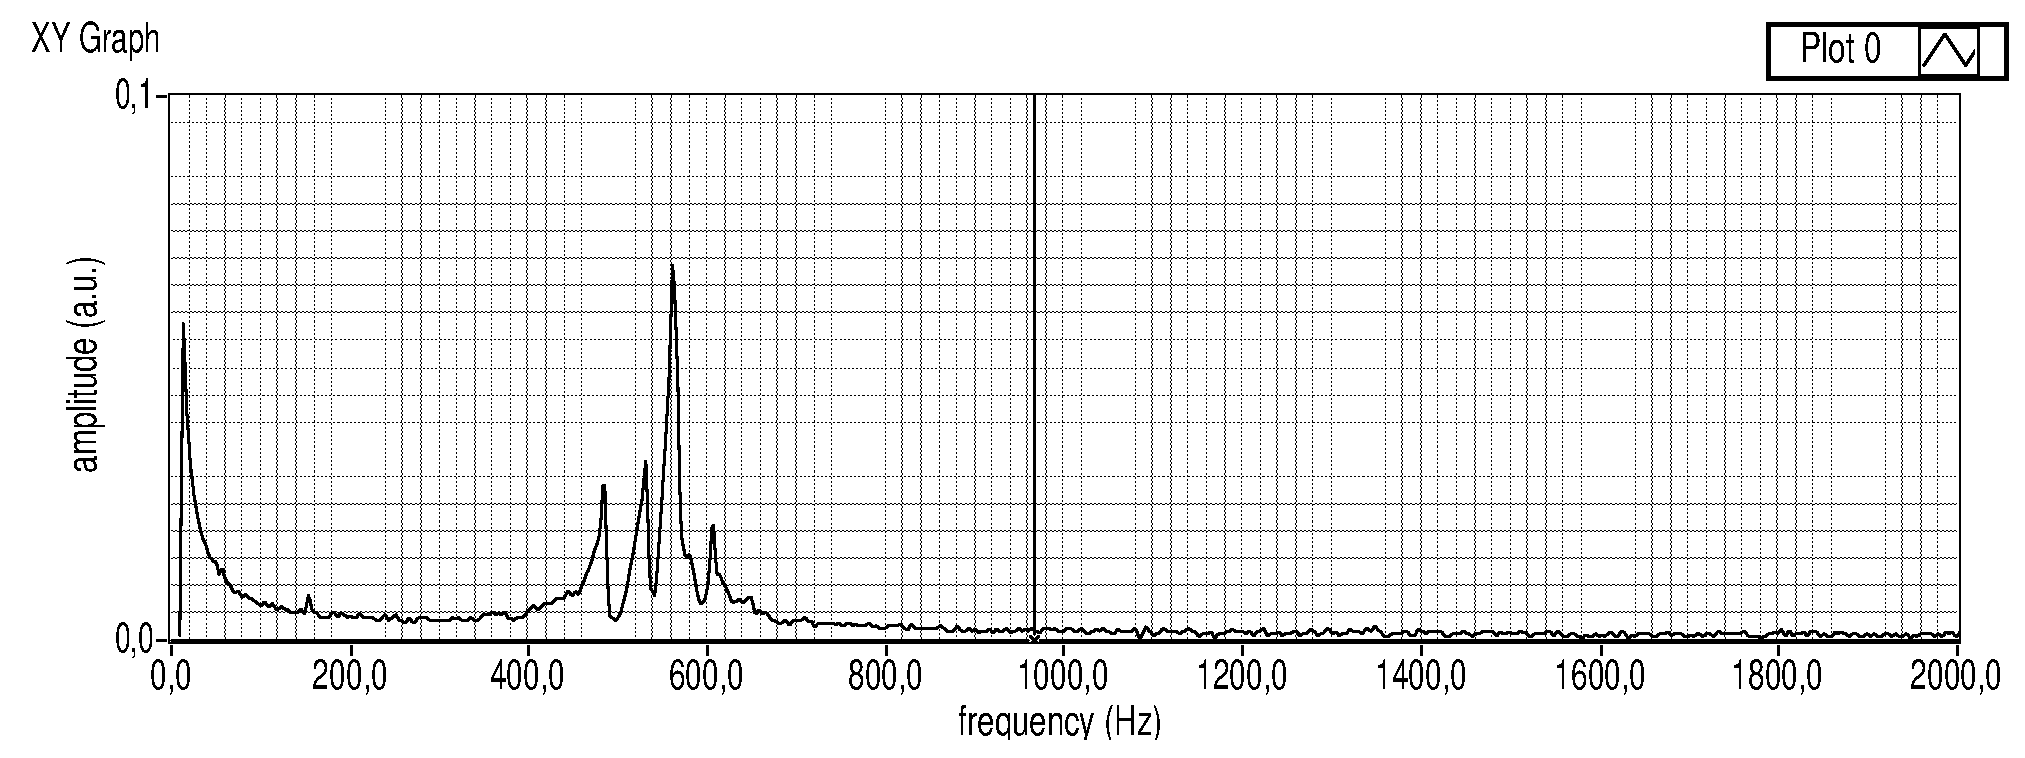
\includegraphics[width=75mm]{A+}
	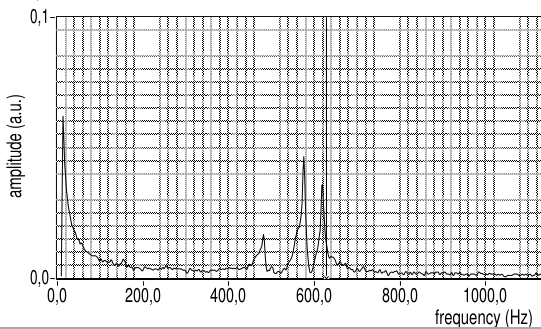
\includegraphics[width=75mm]{B+}
	\caption{\itshape Frequency spectrum of the A+ (left) and of the B+ (right) sample}
	\label{fig:6}
\end{figure}
\noindent
Sample A is from table \ref{tab:2} identified as Fluoroacetone. Fluorine atoms have an odd number of protons and an even number of neutrons in their nucleus such that they possess a nuclear spin of $s=1/2$, this spin can couple in a parallel or antiparallel way with respect to the orientation of the proton´s spin of the $CH_2$ compound, such that we can observe two peaks belonging to $FCH_2$.\cite{Fluorine}



\begin{table}[h]
	\centering
	\begin{tabular}{lllll}
		\toprule
		Peak & frequency $\left[\mathrm{Hz}\right]$ & ppm & difference to TMS & Substance \\
		\midrule
		$ 1$ & $480.0$ & $24.2$ & $6.9$ & Benzene\\
		
		$ 2$ & $574.0$ & $29.0$ &$ 2.1$ & $CH_3$\\
		
		$ 3$ & $616.0$ &$31.1$ & Reference & \\
		\bottomrule
	\end{tabular}
	\caption{Sample B+}
	\label{tab:3}
\end{table}
\noindent
Sample B could either correspond to Toluene or to P-Xylene. By comparison with sample E+ we find the intensity of peak 2 in table \ref{tab:3} to be much larger than its corresponding value of sample E in table \ref{tab:6}, such that we identify sample B as P-Xylene.


\begin{table}[h]
	\centering
	\begin{tabular}{lllll}
		\toprule
		Peak & frequency $\left[\mathrm{Hz}\right]$ & ppm & difference to TMS & Substance \\
		\midrule
		$ 1$ & $386.0$ & $19.5$ & $11.6$ & COOH\\
		
		$ 2$ & $573.9$ & $29.0$ &$ 2.1$ & $CH_3$\\
		
		$ 3$ & $616.0$ &$31.1$ & Reference & \\
		\bottomrule
	\end{tabular}
	\caption{Sample C+}
	\label{tab:4}
\end{table}
\noindent

From table 4 we identify sample C to be Acetic acid.

\begin{figure}[h]
	\centering
	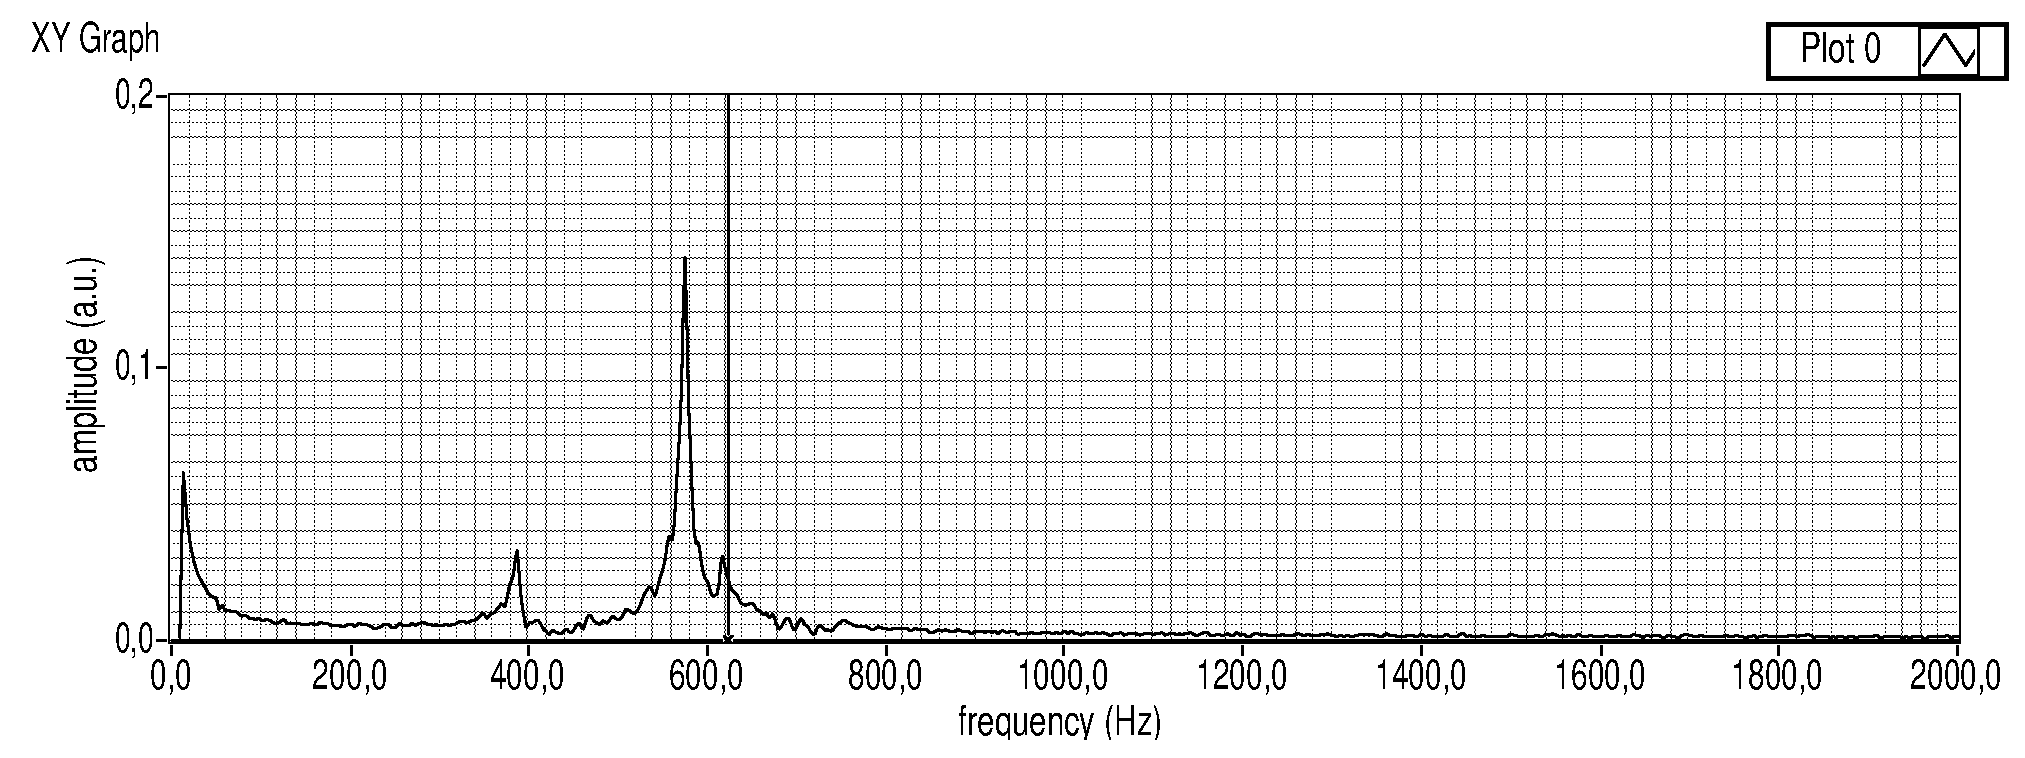
\includegraphics[width=75mm]{C+}
	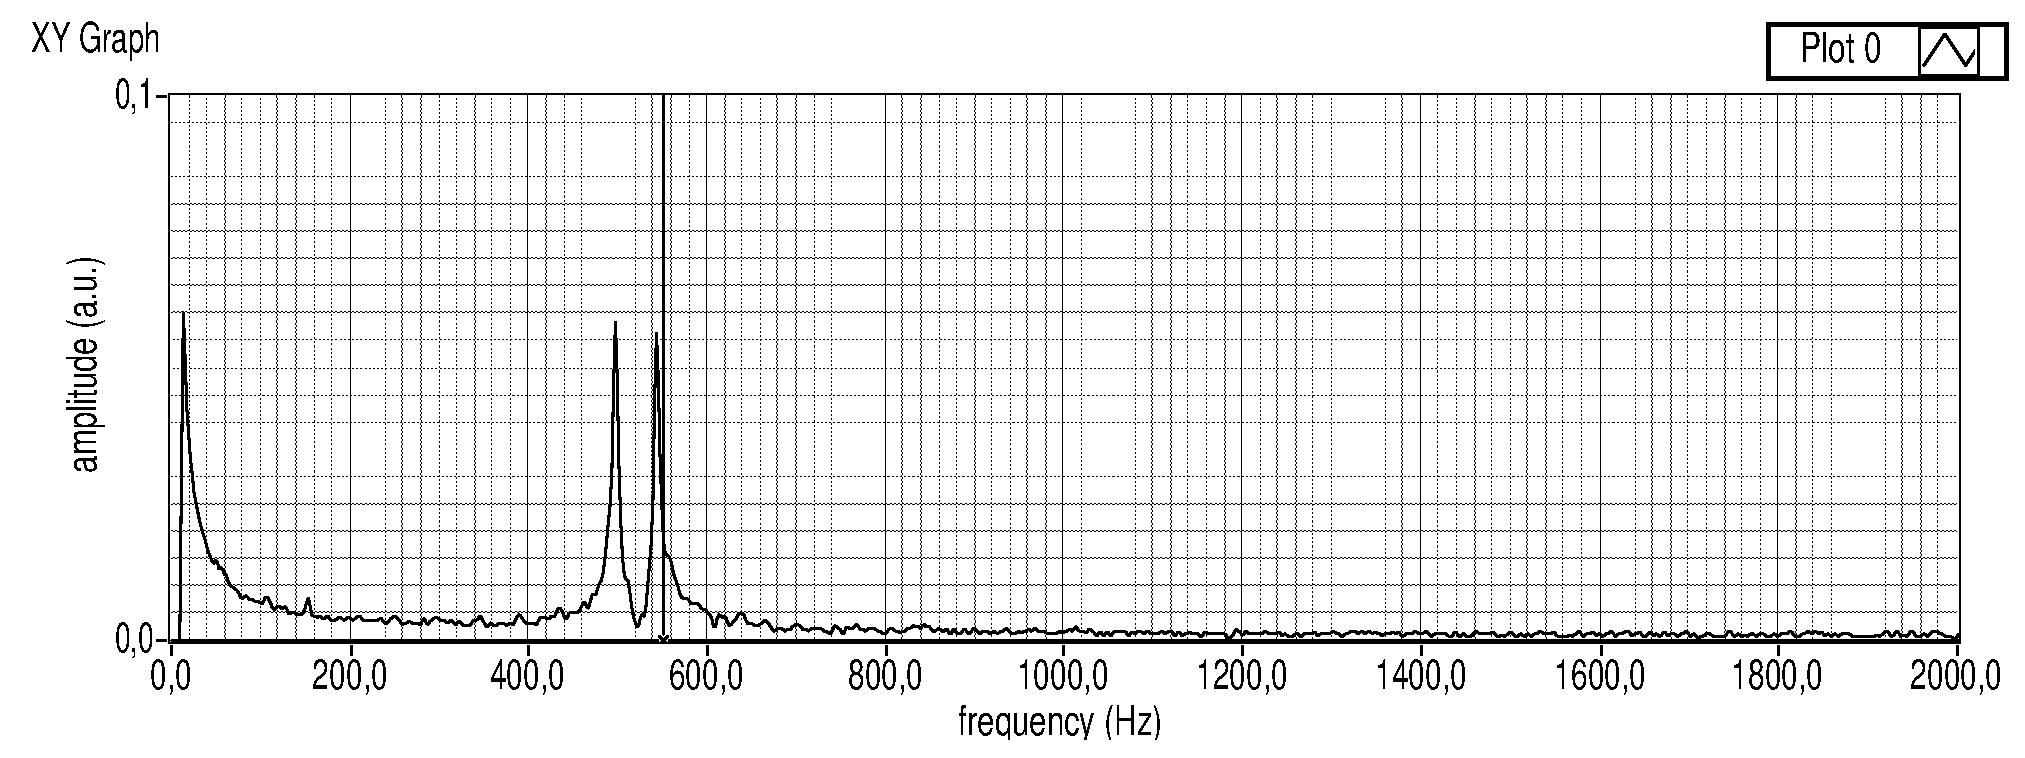
\includegraphics[width=75mm]{D}
	\caption{\itshape Frequency spectrum of the C+(left) and of the D (right) sample}
	\label{fig:8}
\end{figure}
\noindent
\begin{table}[h!]
	\centering
	\begin{tabular}{lllll}
		\toprule
		Peak & frequency $\left[\mathrm{Hz}\right]$ & ppm & difference to TMS & Substance \\
		\midrule
		$ 1$ & $496.0$ & $25.1$ & $6.2$ & $FCH_2$\\
		
		$ 2$ & $ 542.1$ & $27.4$ &$ 3.9$ & $FCH_2$\\
		
		$ 3$ & $31.30 \pm 0.12$ &$31.1$ & Reference from E+, C+, B+ & \\
		\bottomrule
	\end{tabular}
	\caption{Sample D}
	\label{tab:5}
\end{table}

\noindent
As for sample A (compare table \ref{tab:2}) Fluorene couples either in a parallel or antiparallel way with respect to the proton´s spin of the $CH_2$ compound such that we observe two peaks of different frequency corresponding to the same molecule. We therefore identify sample D from table \ref{tab:5} to be Fluoroacetonitril.\\
\begin{table}[h]
	\centering
	\begin{tabular}{lllll}
		\toprule
		Peak & frequency $\left[\mathrm{Hz}\right]$ & ppm & difference to TMS & Substance \\
		\midrule
		$ 1$ & $482.0$ & $24.3$ & $7.1$ & Benzene\\
		
		$ 2$ & $580.0$ & $29.3$ &$ 2.1$ & $CH_3$\\
		
		$ 3$ & $622.0$ &$31.4$ & Reference & \\
		\bottomrule
	\end{tabular}
	\caption{Sample E+}
	\label{tab:6}
\end{table}

\begin{figure}[h]
	\centering
	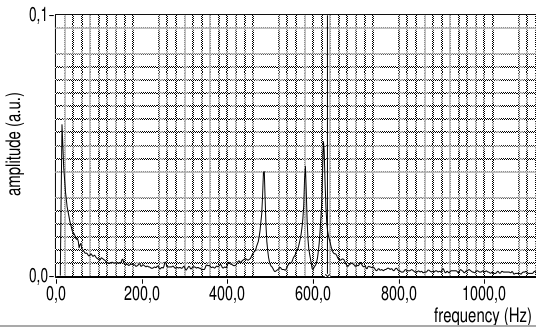
\includegraphics[width=100mm]{E+}
	\caption{\itshape Frequency spectrum of the E+ sample}
	\label{fig:10}
\end{figure}
\noindent
As discussed with sample B+ we identify sample E through comparison with table \ref{tab:3} to be Toluene.

\subsection{Imaging with NMR}
\subsubsection{One dimensional imaging}
The first two samples consisted of two glass tubes filled with 15mm and 50mm of oil respectively. The former sample produced a step function as output signal and the latter sample also  produced a step function but with a broader width. We furthermore observe both samples to show different amplitudes in output signal due to non-linearities of the magnetic field and, furthermore, we observe both signals to be distorted by noise due to making a Fourier transformation of a finite dataset. The resulting images can be seen in figure \ref{fig:11}.
\begin{figure}[h]
	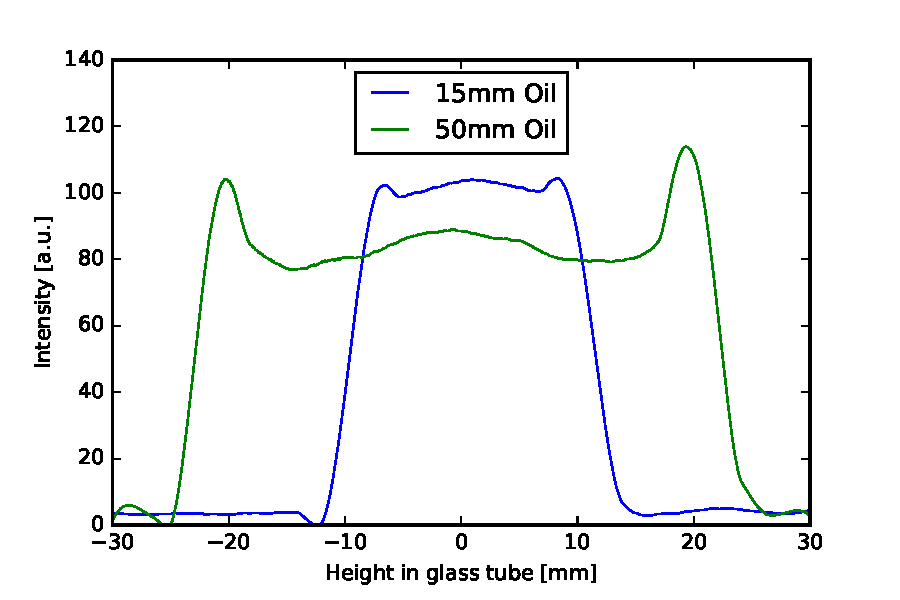
\includegraphics[width=100mm]{1DOilSamples}	
	\centering
	\caption{\itshape 1D imaging of 15 mm and 50 mm oil samples }
	\label{fig:11}
\end{figure}

\noindent
The next sample contained a cylindrical piece of Teflon in the form of seven concentric, similar, equidistant and parallel slices surrounded by oil.
\begin{figure}[h]
	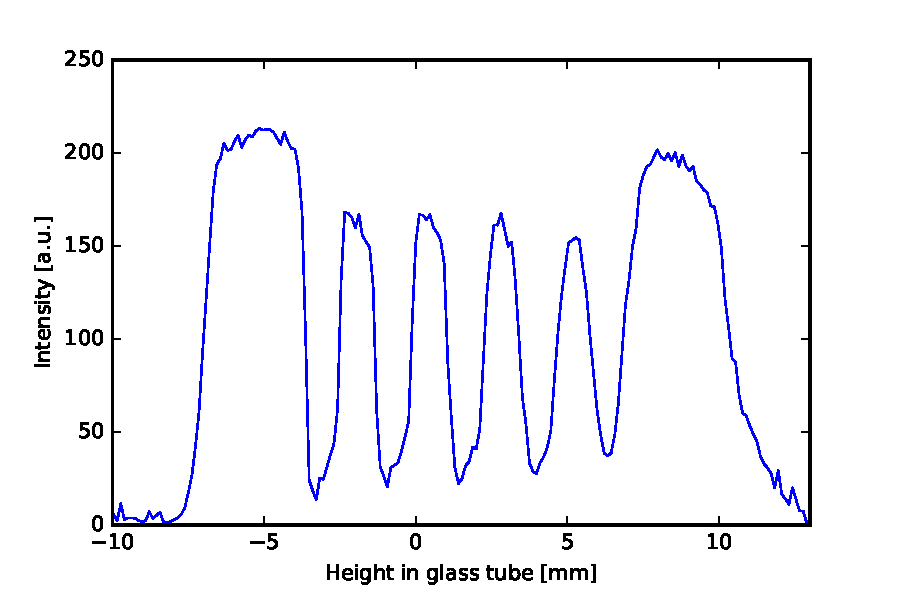
\includegraphics[width=100mm]{OilTef}
	\centering
	\caption{\itshape 1D imaging of an oil sample mixed with Teflon layers}
	\label{fig:12}
\end{figure}
\noindent
 The acquired spectrographic image in figure \ref{fig:12} shows diminished amplitudes in the center of the signal, because the seven slices are connected to a piece of plastic which holds said slices in place and which gives no signal.
 We can furthermore deduce from figure \ref{fig:12}, that the thickness of the Teflon layers ($\approx 1.5 \mathrm{mm}$) is larger than the resolution of the Brucker NMR analyzer mq7.5 used in this setup, otherwise we would simply observe a step function for the whole sample due to the resolution not being high enough to show the oil layers in between the Teflon slices. The resolution of the Bruker NMR analyzer mq7.5 was given by the manual to be $< 1 \mathrm{mm}$. It is limited by the least possible step size of the magnetic field in the measurement being quite large, such that one cannot distinguish in small ranges of B, and by only performing a Fourier transformation of a finite set of datapoints, which in turn results only in an approximate representation of the input signal due to the Fourier transformation of the step function (hyperbolic sine) only having a finite number of main oscillations in the given dataset.
\\
The fourth sample contained 15 mm of sand and approximately 4mm of oil on top. In the following we will answer the question whether this process of oil mixing with sand can be understood as a diffusion process. Figure \ref{fig:13} shows the measured data acquired in steps of 2 minutes in between every plotted line. The signal at first is simply a step-function with some background noise, which represents the input signal from the separated oil layer. The zero point on the x-axis therefore gives us the border between the oil and sand layer. The signal in the $x<0$ area gradually increases over time as the oil sinks more and more into the sand layer. The signal at the end of the mixing process should be a flat, noisy step function as it should represent one signal for the whole oil-sand mixture. We instead observe it not being completely flat, but having some small bumps in between. This is due to tightly bound sand granules in between the mixture which do not let the oil sink through to the bottom side of the glass tube, these areas therefore give no signal.\\
The mixing of oil and sand observed here would describe a diffusion process, if it would fall of like a convex function, compare \cite[(4.24)]{diffusion}: The partial derivative of density with respect to time should be greater than or at least equal to zero. As the diffusion coefficient should be larger than zero, it yields the second derivative of density being larger than or equal to zero, so a convex function. We on the contrary measured this process to fall off in parts like a convex and in parts like a concave function, as seen in figure \ref{fig:13}, such that we cannot deduce solely from this measurement, whether this process actually describes a diffusion process.
\begin{figure}[h]
	\centering
	\includegraphics[width=100mm]{AccumulatedOilSand}
	\caption{\itshape Time dependent evolution of oil sinking into sand}
	\label{fig:13}
\end{figure}

\subsubsection{Two-dimensional imaging}
The first sample consisted of 15mm oil within a glass tube. For horizontal slicing we expected a circle, as the sample gives a signal at every point until the boundaries of the glass tube are met. The result can be seen in figure \ref{fig:14}. The distortion of the circular image to the front is due to non-linearities of the magnetic field intrinsic to this machine, we therefore concluded not to use back to front slicing in the following with this setup.
\begin{figure}[h]
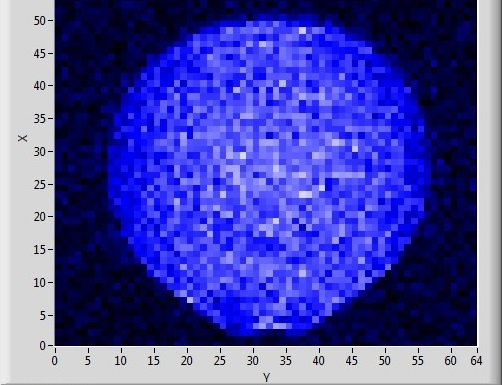
\includegraphics[width=80mm]{OilCircle}
\centering
\caption{\itshape 15mm oil sample sliced back to front horizontally}
\label{fig:14}
\end{figure}
\noindent
\\
We expect a square to show for left to right slicing, again due to the sample consistently giving a signal until the boundaries of the glass tube are met.
The result of the left to right slicing can be seen in figure \ref{fig:15}.
\begin{figure}[h]
	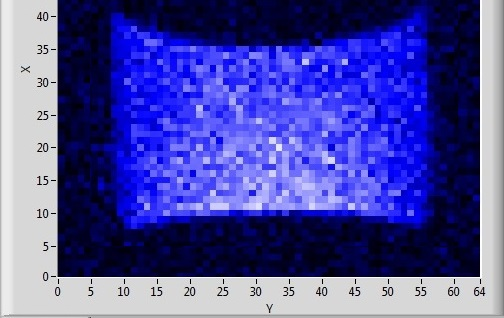
\includegraphics[width=80mm]{OilSlice}
	\centering
	\caption{\itshape 15mm oil sample sliced vertically from left to right }
	\label{fig:15}
\end{figure}  
\noindent
The curve at the top of the slice is due to surface tension  between the oil and the glass tube. The flat edge at the bottom is due to the bottom side of the glass tube.
Throughout the measurement we constantly checked the temperature in the Bruker NMR analyzer mq7.5, it stayed nearly constant and only changed by 0.001 \textcelsius.\\
\label{sec:4}

\noindent
We proceeded with taking 2D images of organic objects.\\
Figure \ref{fig:16} shows a peanut with shell. We can only observe one nut (the dark, elliptical object inside the upper cell), because the peanut was not completely centered in the glass tube such that the left to right slice only slices through one of the cells (the upper one with the nut shown) and only captures the beginning of the lower cell as the slice went right through the middle between the two cells.
\begin{figure}[h]
	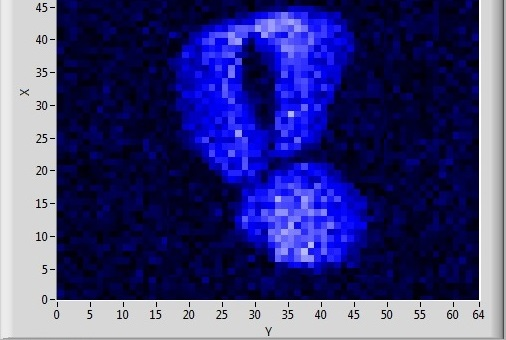
\includegraphics[width=80mm]{Peanut}
	\centering
	\caption{\itshape Peanut inside shell sliced vertically from left to right}
	\label{fig:16}
\end{figure}
\begin{figure}[h]
	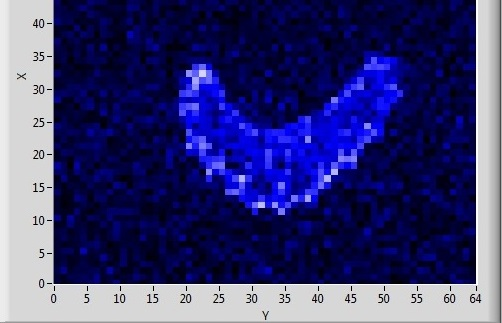
\includegraphics[width=80mm]{Celery}
	\centering
	\caption{\itshape Sample of celery sliced horizontally}
	\label{fig:17}
\end{figure}
\noindent
\\
Figure \ref{fig:17} shows the C-shaped form of a piece of celery. This is the second image taken from the same sample as the first one only showed unidentifiable structure, because here no perfect gradient could be calibrated due to the sample not being placed perfectly inside the measurement boundaries of the Bruker NMR analyzer mq7.5. 

\noindent
Figure \ref{fig:18} in contrast shows an apple core sliced horizontally. The star shaped core contains apple seeds which do not give any signal, hence the black areas. The signal of the area around the core comes from the pulp around it, it was partially cut off such that the shown shape is not perfectly circular.
\begin{figure}[h]
	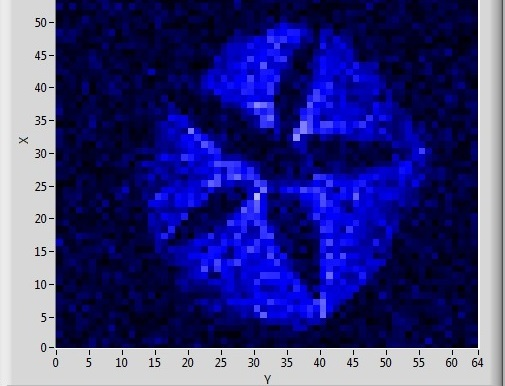
\includegraphics[width=80mm]{Apple}
	\centering
	\caption{\itshape Sample of an apple core sliced horizontally}
	\label{fig:18}
\end{figure}